\documentclass[11pt, a4paper,spanish]{article}

\usepackage[T1]{fontenc}
\usepackage[hmarginratio=1:1,top=26mm]{geometry}


\usepackage{graphicx}
\graphicspath{ {images/} }

\usepackage{dirtytalk}

\usepackage{fancyhdr}
\pagestyle{fancy}
\fancyhead{}
\fancyfoot{}
\fancyhead[C]{ \today \ $\bullet$ Ingeniería del Conocimiento $\bullet$ Tutoría sobre Programación Lógica}
\fancyfoot[RO]{\thepage}

%-------------------------------------------------------------------------------
%	TITLE SECTION
%-------------------------------------------------------------------------------

\title{\vspace{-15mm}\fontsize{24.88pt}{10pt}\textbf{Tutoría sobre Programación Lógica}} % Article title

\author{Sergio García Prado}
\date{\today}

%-------------------------------------------------------------------------------

\begin{document}

	\maketitle % Insert title

	\thispagestyle{fancy} % All pages have headers and footers

%-------------------------------------------------------------------------------
%	TEXT
%-------------------------------------------------------------------------------

	\section{Sea $P$ el programa normal: \\
		$\{animal(snoopy) \gets, \\
		animal(kitty) \gets, \\
		gatito(kitty) \gets, \\
		gusta(elena,x) \gets animal(x), \neg gatito(x)\}\\$
		y $G$ la meta: \\
		$\gets \neg gusta(elena,kitty)$\\
		?`Cuál es la respuesta computada de $P \cup {G}$ ?}

		\paragraph{}


	\section{Elaborar un programa definido que junto a la meta $G$: $\gets p(x,y)$ tenga como respuestas correctas $\{ a / x \}$ y $\{b / y\}$ pero no $\{c / x, d / y\}$, con la restricción de que el símbolo de predicado p no ocurra en ningún hecho.}

		\paragraph{}
		Conjunto de hechos y reglas:
		\[ f(a) \gets, \]
		\[ f(b) \gets, \]
		\[ p(x,y) \gets f(x), f(y) \]

		\paragraph{}
		Puesto que estamos elaborando un programa definido, que por definición es un  \say{conjunto de hechos y reglas que describen explícitamente qué es cierto, sin información explicita sobre qué es falso}, no tenemos que indicar nada sobre las constantes $c$ y $d$.

	\clearpage
	\section{Sea $P$ el programa definido: \\
		$\{entero(0) \gets ,\\
		entero(x) \gets entero(y), =(x, +(y,1))\}\\$
		y $G$ la meta: \\
		$\gets entero(2)$\\
		Obtener las tres secuencias de un cómputo de G por P que obtenga la meta vacía.}

		\paragraph{}
		Para obtener la meta vacía se llevará a cabo una resolución SLD con la selección del primer literal de la cláusula como regla de cómputo y busqueda primero en profundidad como regla de búsqueda. El cómputo por tanto queda de la siguiente manera. Las secuencias de cómputo son:
		\begin{itemize}
			\item Metas: $G_0, G_1, G_2,G_3$
			\item Cláusulas: $C_1, C_2,C_3$
			\item UMG's $O_1, O_2, O_3$
		\end{itemize}
		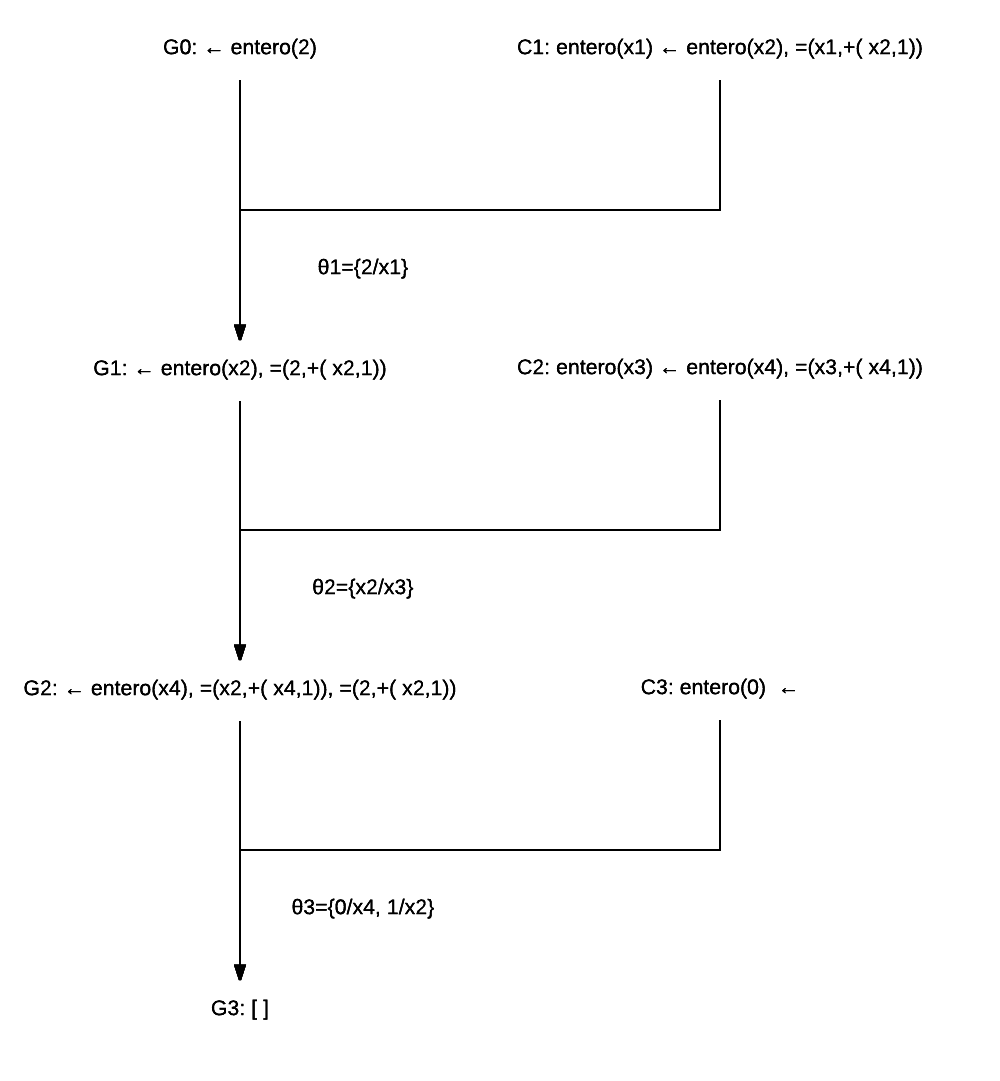
\includegraphics[width=0.9\textwidth]{sld-computation}

\end{document}
